% Created 2024-07-08 Mon 22:16
% Intended LaTeX compiler: pdflatex
\documentclass[11pt]{article}
\usepackage[utf8]{inputenc}
\usepackage[T1]{fontenc}
\usepackage{ragged2e}
\usepackage{caladea}
\usepackage{graphicx}
\usepackage{longtable}
\usepackage{wrapfig}
\usepackage{rotating}
\usepackage[normalem]{ulem}
\usepackage{amsmath}
\usepackage{amssymb}
\usepackage{capt-of}
\usepackage{hyperref}
\usepackage{fancyhdr}
\title{Novena à Santa Bibiana}
 % \hypersetup{
 %  pdfauthor={},
 %  pdftitle={Novena a/à SANTO_NOME},
 %  pdfkeywords={},
 %  pdfsubject={},
 %  pdfcreator={Emacs 29.4 (Org mode 9.6.15)}, 
 %  pdflang={English}
 % }

\title{
  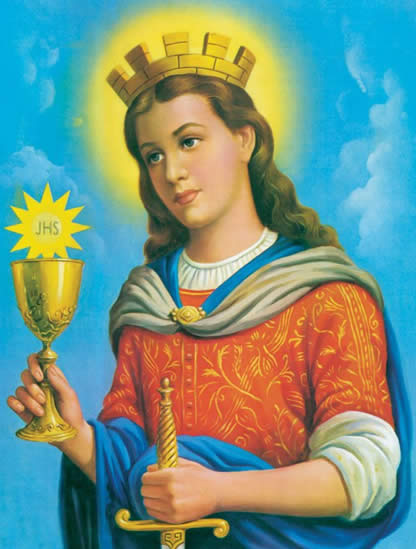
\includegraphics[scale=0.7]{./assets/imagem.jpg}
  \par
  NOVENA A SANTA BÁRBARA}
\author{Garamog, Nina Freitas}
\date{24/11 - 03/12}
\renewcommand{\contentsname}{Sumário}

\begin{document}


\maketitle

\pagestyle{fancy}
\fancyhf{} % clear existing header/footer entries
\fancyfoot[LO, CE]{
  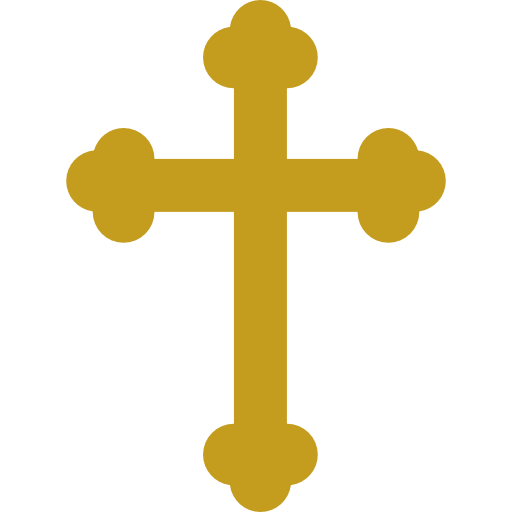
\includegraphics[scale=0.2]{./assets/cross.png} Santa Bárbara, Rogai por Nós!
}
% Place Page X of Y on the right-hand
% side of the footer
\fancyfoot[R]{\thepage}
  
\newpage

\tableofcontents

\centering
\vfill
Visite-nos no Telegram: \url{https://t.me/CotidieNovena}
\newpage


\section{História}\label{historia}


\begin{justify}



  \par Santa Bárbara nasceu na cidade de Nicomédia na região da Bitínia, onde hoje se localiza a cidade de Izmit, na Turquia, às margens do Mar de Mármara. Bárbara viveu no final do Século III. Foi uma bela jovem, filha única de Dióscoro, um rico e nobre morador de Nicomédia.

Dióscoro não queria deixar sua filha única viver no meio da sociedade corrupta daquele tempo. Por isso, decidiu fechá-la numa torre. Lá, ela era ensinada por tutores da confiança de seu pai. Porém, aquilo que parecia um castigo, começou a abrir a mente de Bárbara. Do alto da torre ela contemplou a natureza: as estações do ano, a chuva, o sol, a neve, o frio, o calor, as aves, os animais, etc. Tudo isso fez Bárbara questionar se aquilo era realmente criação dos "deuses", como seus tutores e seu povo creditavam, ou se havia "alguém" muito mais inteligente e poderoso por trás da criação.

\subsection{A beleza de divina}

Quando atingiu a idade para o casamento, por volta de 17 anos, seu pai a trouxe para casa e permitia que ela recebesse a visita de pretendentes, mas não permitia que ela visitasse a cidade. Bárbara era uma jovem muito bela e de família rica. Por isso, muitos eram os pretendentes que queriam se casar com ela. Mas Bárbara não aceitava nenhum, enxergando neles a superficialidade e o interesse, e nenhum toque de amor verdadeiro.

Para seu pai, isso era um problema sério, pois, segundo os costumes, ele tinha obrigação de casar sua filha. Dióscoro pensava que as "desfeitas" da filha diante dos pretendentes se davam por causa do tempo que ela passou na torre. Então, ele decidiu permitir que Bárbara conhecesse a cidade.

\subsection{O contato com os cristãos}

Santa Bárbara, então, começou a frequentar a cidade. Nessas visitas, acabou conhecendo os cristãos de Nicomédia. Estes passaram para Bárbara a mensagem de Jesus Cristo. Falaram-lhe também sobre o mistério da Santíssima Trindade. A novidade cristã tocou profundamente o coração de Bárbara. Com os cristãos ela encontrou a resposta para seus questionamentos: o Criador de tudo era o Deus Único e Pai de Nosso Senhor Jesus Cristo e não os deuses que seu povo cultuava.

Bárbara se converteu ao cristianismo de todo o coração. Logo, um padre vindo de Alexandria ministrou a ela o batismo. E Bárbara passou a ser uma jovem fervorosa e cheia de virtudes cristãs. Em Jesus Cristo ela encontrou o sentido mais profundo de sua vida.

\subsection{Santa Bárbara e as perseguições}

Dióscoro, pai de Santa Bárbara, decidiu construir para ela uma casa de banho na torre, onde ele planejou instalar duas belas janelas. Quando a obra começou, Dióscoro teve que fazer uma longa viagem. Durante a viagem do pai, Santa Bárbara ordenou que construíssem uma terceira janela na obra. Sua intenção era que a torre tivesse três janelas em homenagem à Santíssima Trindade. Além disso, Santa Bárbara esculpiu uma cruz na torre.

Quando Dióscoro voltou, reparou logo nas mudanças feitas na construção e foi perguntar à filha o por que daquilo. Santa Bárbara explicou que as mudanças eram símbolos de sua nova fé: três janelas em homenagem ao Deus Uno e Trino, Criador de todas as coisas. E a Cruz lembrava o sacrifício do Filho de Deus para salvar a humanidade. Dióscoro ficou furioso.

\subsection{A sentença de morte de Santa Bárbara}

Ao perceber que a filha estava irredutível em sua fé cristã, Dióscoro, num impulso de ira, denunciou a filha ao prefeito da cidade. Este ordenou que Bárbara fosse torturada em praça pública, para tentar fazer com que a jovem renegasse a fé cristã. Porém, para surpresa de todos, Santa Bárbara não renegou sua fé, mesmo diante dos mais atrozes sofrimentos.

Durante a tortura, uma jovem cristã chamada Juliana denunciou os nomes dos carrascos, coisa que era expressamente proibida na época. Por isso, Juliana foi presa e condena à morte por decapitação juntamente com Santa Bárbara.

As duas jovens cristãs foram levadas amarradas pelas ruas de Nicomédia, sob os gritos furiosos de muita gente. Santa Bárbara teve os seios cortados. Depois, foi conduzida para fora da cidade. Lá, seu próprio pai a degolou.

\subsection{Bárbara e os raios}

Quando Dióscoro degolou a filha e a cabeça de Santa Bárbara rolou pelo chão, um raio riscou o céu e um enorme trovão foi ouvido pelo povo. E, para o assombro de todos, o corpo de Dióscoro caiu no chão sem vida, atingido pelo raio. Parece que a natureza se revoltou contra a atitude desse pai infanticida.

Depois deste fato, Santa Bárbara ganhou o status de 'protetora contra relâmpagos e tempestades', além de ser nomeada Padroeira dos artilheiros, dos mineradores e das pessoas que trabalham com fogo.

\subsection{Devoção à Santa Bárbara}

A festa de Santa Bárbara é celebrada na Igreja Católica e na Igreja Ortodoxa. A festa é celebrada no dia 4 de Dezembro de cada ano.

Mas a grande mensagem de Santa Bárbara destina-se a todos aqueles que buscam a verdade, principalmente os jovens. Ela nos ensina a buscar a verdade com coração sincero e aberto. Ensina também que o casamento não deve acontecer por mero interesse, mas sim por amor. Por fim, Santa Bárbara nos dá uma mensagem de coragem e fé. A palavra mártir quer dizer testemunha e se aplica aos cristãos que preferiram morrer a negar sua fé e pecar. Este é o grande testemunho de Santa Bárbara.
Oração de Santa Bárbara

"Santa Bárbara, que sois mais forte que as torres das fortalezas e a violência dos furacões, fazei que os raios não me atinjam, os trovões não me assustem e o troar dos canhões não me abalem a coragem e a bravura. Ficai sempre ao meu lado para que possa enfrentar de fronte erguida e rosto sereno todas as tempestades e batalhas de minha vida, para que, vencedor de todas as lutas, com a consciência do dever cumprido, possa agradecer a vós, minha protetora, e render graças a Deus, criador do céu, da terra e da natureza: este Deus que tem poder de dominar o furor das tempestades e abrandar a crueldade das guerras. Por Cristo, nosso Senhor. Amém."

\end{justify}
Amém!

\subsection*{Créditos }
\href{https://cruzterrasanta.com.br/historia-de-santa-barbara/64/102/}{Cruz Terra Santa}

\newpage
\section{Orações}\label{oracoes}

\subsection{Oração a Santa Bárbara}

Senhor, que escolhestes Santa Bárbara para consolar os vivos e os moribundos, concedei-nos que vivamos sempre no vosso divino amor e ponhamos toda a nossa esperança nos merecimentos da dolorosíssima Paixão de vosso Filho, a fim de que a morte não nos colha em estado de pecado mortal, mas que, munidos dos santos Sacramentos da penitência, eucaristia e unção, possamos caminhar sem temor para a glória eterna. Nós vo-lo pedimos pelo mesmo Jesus Cristo, Nosso Senhor. Assim seja.

\textbf{Pai-Nosso, Avé-Maria e Glória.}

\subsection{Créditos:}
\href{https://www.nadateespante.com/products/novena-a-santa-barbara-para-sermos-preserverados-da-morte-repentina-ou-imprevista-/}{Nada Te Espante}


\end{document}
